\section{Auswertung}
\label{sec:Auswertung}



\subsection{Die $U/I$-Graphen der verschiedenen Spannungsquellen}

\subsubsection{Gleichspannungsquelle}
\begin{figure}[H]
	\centering
	\caption{}
	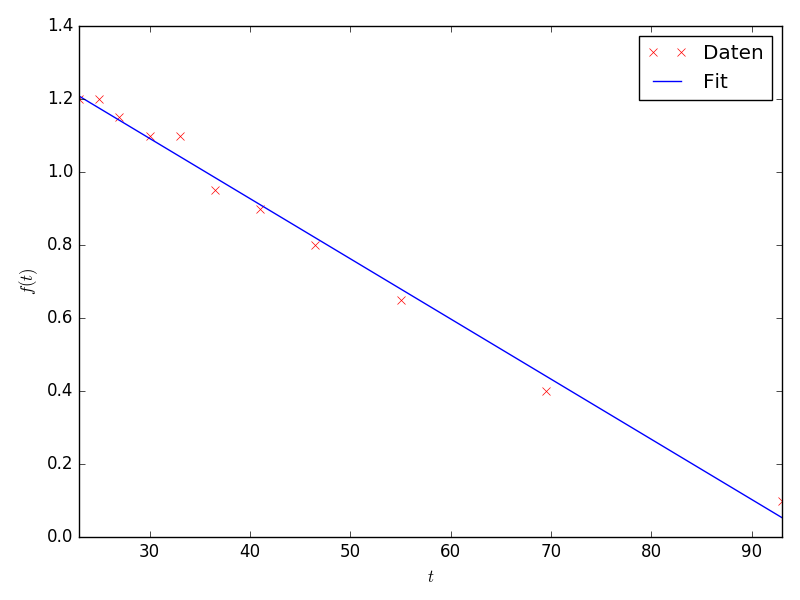
\includegraphics[width=\linewidth-70pt,height=\textheight-70pt,keepaspectratio]{Gleichstrom.png}
	\label{fig:Gleichstrom}
\end{figure}
\begin{table}
	\centering
	\caption{Ergebnisse der Gleichstrommessung ohne Gegenspannung}
	\label{tab:Gleichstrom}
	\sisetup{table-format=1.2}
	\begin{tabular}{S S }
		\toprule
		{$I/$mA} & {$U_k/$V} \\
		\midrule
		23.0 & 1.20 \\
		25.0 & 1.20 \\
		27.0 & 1.15 \\
		30.0 & 1.10 \\
		33.0 & 1.10 \\
		36.5 & 0.95 \\
		41.0 & 0.90 \\
		46.5 & 0.80 \\
		55.0 & 0.65 \\
		69.5 & 0.40 \\
		93.0 & 0.10 \\
		\bottomrule
	\end{tabular}
\end{table}


\newpage
\subsubsection{Gleichspannungsquelle mit Gegenspannung}

\begin{figure}[H]
	\centering
	\caption{}
	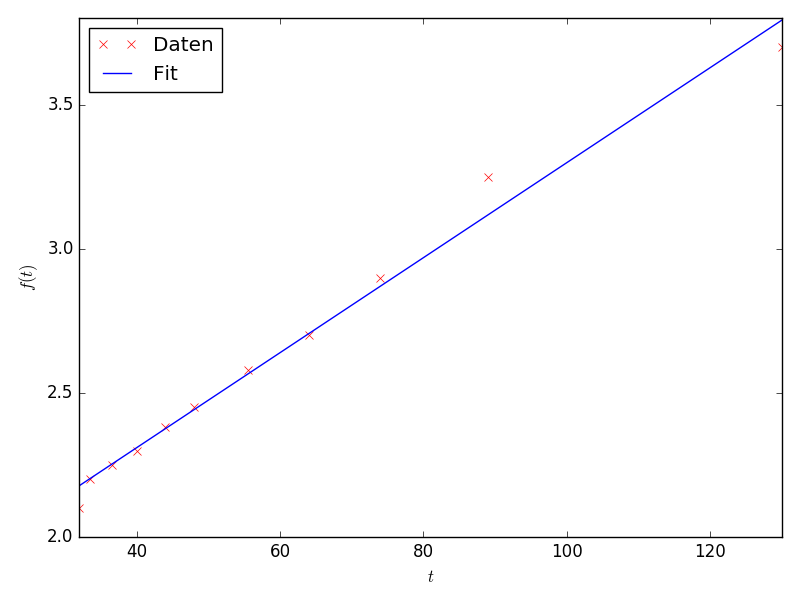
\includegraphics[width=\linewidth-70pt,height=\textheight-70pt,keepaspectratio]{GleichstromR.png}
	\label{fig:GleichstromR}
\end{figure}
\begin{table}
	\centering
	\caption{GleichstromR}
	\label{tab:GleichstromR}
	\sisetup{table-format=1.2}
	\begin{tabular}{S S }
		\toprule
		{$I/mA$} & {$U/V$} \\
		\midrule
		32.0 & 2.1 \\
		33.5 & 2.2 \\
		36.5 & 2.25 \\
		40.0 & 2.3 \\
		44.0 & 2.38 \\
		48.0 & 2.45 \\
		55.5 & 2.58 \\
		64.0 & 2.7 \\
		74.0 & 2.9 \\
		89.0 & 3.25 \\
		130.0 & 3.7 \\
		\bottomrule
	\end{tabular}
\end{table}

\newpage
\subsubsection{Rechteck-Spannungsquelle}

\begin{figure}[H]
	\centering
	\caption{}
	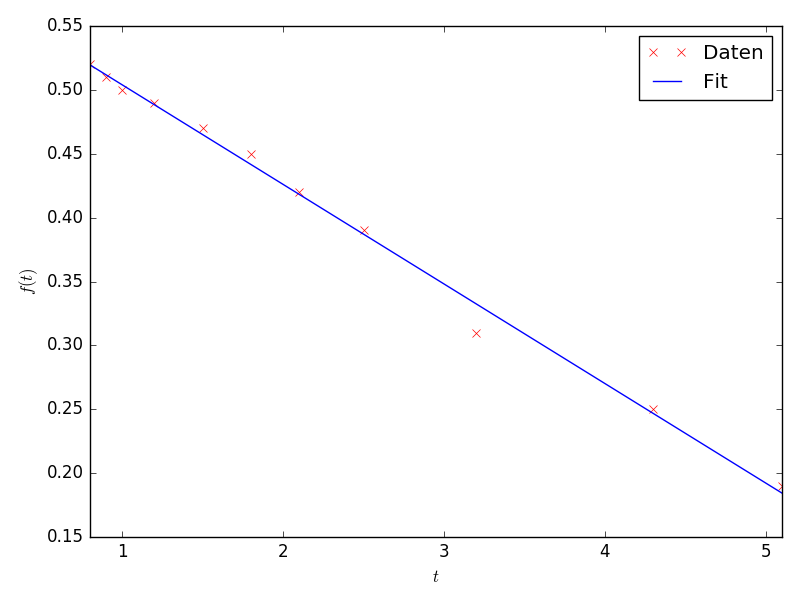
\includegraphics[width=\linewidth-70pt,height=\textheight-70pt,keepaspectratio]{Rechteck.png}
	\label{fig:Rechteck}
\end{figure}
\begin{table}
	\centering
	\caption{Rechteck}
	\label{tab:Rechteck}
	\sisetup{table-format=1.2}
	\begin{tabular}{S S }
		\toprule
		{$I/mA$} & {$U/V$} \\
		\midrule
		0.8 & 0.52 \\
		0.9 & 0.51 \\
		1.0 & 0.5 \\
		1.2 & 0.49 \\
		1.5 & 0.47 \\
		1.8 & 0.45 \\
		2.1 & 0.42 \\
		2.5 & 0.39 \\
		3.2 & 0.31 \\
		4.3 & 0.25 \\
		5.1 & 0.19 \\
		\bottomrule
	\end{tabular}
\end{table}

\newpage
\subsubsection{Sinus-Spannungsquelle}

\begin{figure}[H]
  \centering
  \caption{}
  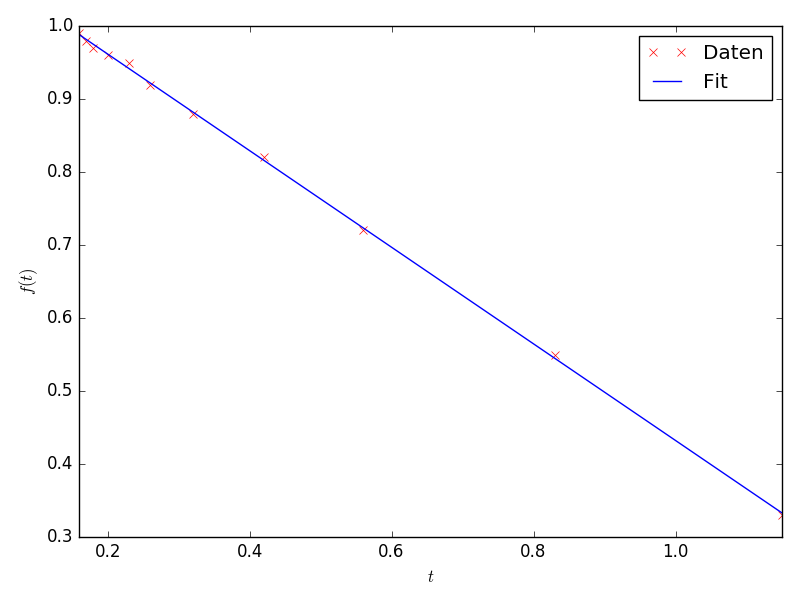
\includegraphics[width=\linewidth-70pt,height=\textheight-70pt,keepaspectratio]{Sinus.png}
  \label{fig:Sinus}
\end{figure}
\begin{table}
	\centering
	\caption{Sinus}
	\label{tab:Sinus}
	\sisetup{table-format=1.2}
	\begin{tabular}{S S }
		\toprule
		{$I/mA$} & {$U/V$} \\
		\midrule
		0.16 & 0.99 \\
		0.17 & 0.98 \\
		0.18 & 0.97 \\
		0.2 & 0.96 \\
		0.23 & 0.95 \\
		0.26 & 0.92 \\
		0.32 & 0.88 \\
		0.42 & 0.82 \\
		0.56 & 0.72 \\
		0.83 & 0.55 \\
		1.15 & 0.33 \\
		\bottomrule
	\end{tabular}
\end{table}

\newpage
\subsection{Die lineare Ausgleichsrechnung zu den Messwerten}
Um die Ausgleichsgerade $f(x)=ax+b$ zu berechnen werden folgende Formeln verwendet:

\begin{equation}
a=\frac{ \overline{xy} - \overline{x} \cdot \overline{y}}{\overline{x^2} - \overline{x}^2}
\end{equation}
\begin{equation}
b=\frac{\overline{x^2} \cdot \overline{y} - \overline{x} \cdot \overline{xy}}{\overline{x^2} - \overline{x}^2}\text{.}
\end{equation}
Und um die Standartabweichung der ermittelten Parameter zu bestimmen werden folgende Formeln verwendet:
\begin{equation}
\sigma_y=\sqrt{\frac{1}{N-2}\sum\limits_{i=1}^{N}(y_i - a x_i - b)^2}
\end{equation}
\begin{equation}
\sigma_a=\sqrt{\frac{\sigma_y^2}{N ( \overline{x^2} - \overline{x} ^2 )}}
\end{equation}
\begin{equation}
\sigma_b=\sqrt{\frac{\sigma_y^2 \cdot \overline{x}}{N ( \overline{x^2} - \overline{x} ^2 )}}\text{.}
\end{equation}
$\sigma_y$ ist hier die Standartabweichung der $y$-Werte von der ermittelten Ausgleichsgeraden.


\subsubsection{Ausgleichsrechnung für die Messwerte der Messung mit Gleichspannungsquelle}
Mit den Formeln (5) und (6) und den Werten aus Tabelle 1 folgt:
\begin{displaymath}
	a=-0,01650
\end{displaymath}
\begin{displaymath}
	b=1,59\text{.}
\end{displaymath}
Damit ergibt sich mit Formel (7):
\begin{displaymath}
	\sigma_y=0,03
\end{displaymath}
und mit den Formeln (8) und (9):
\begin{displaymath}
	\sigma_a=0,00050
\end{displaymath}
\begin{displaymath}
	\sigma_b=0,02\text{.}
\end{displaymath}
Hieraus folgt nach Formel (1):
\begin{displaymath}
	R_i=16,50\text{ }\Omega\pm 0,50\text{ }\Omega
\end{displaymath}
\begin{displaymath}
	U_0=1,59\text{ V}\pm 0,02\text{ V.}
\end{displaymath}

\subsubsection{Ausgleichsrechnung für die Messwerte der Messung mit Gleichspannungsquelle und Gegenspannung}

Mit den Formeln (5) und (6) und den Werten aus Tabelle 2 folgt:
\begin{displaymath}
a=0,01648
\end{displaymath}
\begin{displaymath}
b=1,65\text{.}
\end{displaymath}
Damit ergibt sich mit Formel (7):
\begin{displaymath}
\sigma_y=0,06
\end{displaymath}
und mit den Formeln (8) und (9):
\begin{displaymath}
\sigma_a=0,00065
\end{displaymath}
\begin{displaymath}
\sigma_b=0,04\text{.}
\end{displaymath}
Hieraus folgt nach Formel (4):
\begin{displaymath}
R_i=16,48\text{ }\Omega\pm 0,65 \text{ }\Omega
\end{displaymath}
\begin{displaymath}
U_0=1,65\text{ V}\pm 0,04\text{ V.}
\end{displaymath}

\subsubsection{Ausgleichsrechnung für die Messwerte der Messung mit Rechteck-Spannungsquelle}
Mit den Formeln (5) und (6) und den Werten aus Tabelle 3 folgt:
\begin{displaymath}
a=-0,07798
\end{displaymath}
\begin{displaymath}
b=0,582\text{.}
\end{displaymath}
Damit ergibt sich mit Formel (7):
\begin{displaymath}
\sigma_y=0,009
\end{displaymath}
und mit den Formeln (8) und (9):
\begin{displaymath}
\sigma_a=0,00191
\end{displaymath}
\begin{displaymath}
\sigma_b=0,005\text{.}
\end{displaymath}
Hieraus folgt nach Formel (1):
\begin{displaymath}
R_i=77,98\text{ }\Omega\pm 1,91\text{ }\Omega
\end{displaymath}
\begin{displaymath}
U_0=0,582\text{ V}\pm 0,005\text{ V.}
\end{displaymath}

\subsubsection{Ausgleichsrechnung für die Messwerte der Messung mit Sinus-Spannungsquelle}
Mit den Formeln (5) und (6) und den Werten aus Tabelle 4 folgt:
\begin{displaymath}
a=-0,66185
\end{displaymath}
\begin{displaymath}
b=1,094\text{.}
\end{displaymath}
Damit ergibt sich mit Formel (7):
\begin{displaymath}
\sigma_y=0,004
\end{displaymath}
und mit den Formeln (8) und (9):
\begin{displaymath}
\sigma_a=0.00432
\end{displaymath}
\begin{displaymath}
\sigma_b=0,002\text{.}
\end{displaymath}
Hieraus folgt nach Formel (1):
\begin{displaymath}
R_i=661,85\text{ }\Omega\pm 4,32\text{ }\Omega
\end{displaymath}
\begin{displaymath}
U_0=1,094\text{ V}\pm 0,002\text{ V.}
\end{displaymath}
























































\subsection{Der systematische Fehler einer unmittelbaren $U_0$-Bestimmung mit einem Voltmeter}
Der systematische Fehler einer unmittelbaren Leerlaufspannungsermittlung folgt aus der Näherung, dass
der Innenwiderstand des Voltmeters unendlich betrage. Da dies bei einem realen Voltmeter nicht der
Fall ist kommt es zu einem systematischen Fehler.
Aus der Formel (1) ergibt sich sofort
\begin{equation}
U_0 = \frac{U_k}{R_v}(R_v + R_i)
\end{equation}
und daraus der absolute systematische Fehler
\begin{equation}
\Delta U = \frac{U_k}{R_v}R_i \text.
\end{equation}
Es ergibt sich ein systematischer Fehler von $2,64 \cdot 10^{-6} $ V.





\subsection{Der systematische Fehler aufgrund einer falschen Platzierung des Voltmeters}
Auch die falsche Positionierung des Voltmeters im Stromkreis führt zu einem
systematischen Fehler. Fügt man das Voltmeter wie in Abbildung 2 an der Stelle H
ein, also hinter dem Amperemeter, müsste man dessen kleinen, aber durchaus existenten
Innenwiderstand miteinbeziehen.

\newpage
\subsection{Leistungsanpassung einer Monozelle}
Trägt man die mit Formel (4) bestimmte Leistung gegen $R_a = U_k/I$ auf erhält man
den folgenden Graphen:
\begin{figure}[H]
	\centering
	\caption{}
	\includegraphics[width=\linewidth-150pt,height=\textheight-150pt,keepaspectratio]{GleichstromRe.png}
	\label{fig:GleichstromLeistung}
\end{figure}
Beim Vergleich mit der Theoriekurve nach Formel (3) fällt auf, dass die Messergebnisse zwar schwanken, sich jedoch höchstens eine kleine Tendenz nach unten feststellen lässt. Somit liegen die Punkte haupsächtlich im Rahmen der Messungenauigkeit.
